\chapter{Experiments}
 
\section{Experiment 1}
The first experiment was conducted on a fully synthetic dataset. Supervised and unsupervised learning approaches were used to detect the anomalies. 

\subsection{Dataset} \label{dataset1}
The dataset, that was created for this first task consisted of five variables. The dataset was created under the assumption, that one measurement was drawn per hour on totally 2000 days, resulting in 48000 datapoints. The variables all follow a cyclic pattern shown in figure \ref{fig:synthetic data} but are not dependent on each other. 

\begin{figure}[h]
	\centering
	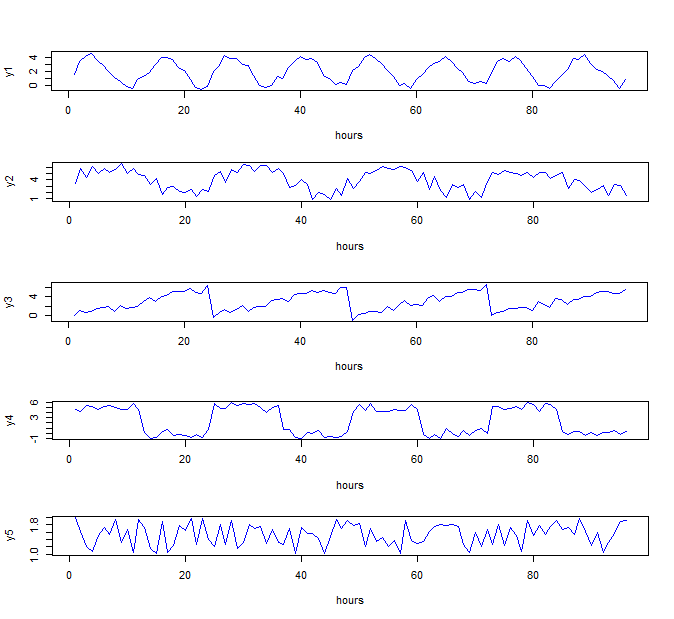
\includegraphics[scale=0.7]{Figures/synthetic data}
	\decoRule
	\caption[Synthetic Dataset]{Synthetic Dataset \parencite{own}}
	\label{fig:synthetic data}
\end{figure}

In a second step the dataset was enriched with six different kinds of anomalies. The anomalies embedded into the dataset are of type deviant cycle, temporary change and level shift. Figure \ref{fig:anomalies} shows examples of the embedded anomalies. The same kind of anomalies were embedded into the training and the test dataset.

\begin{figure}[h]
	\centering
	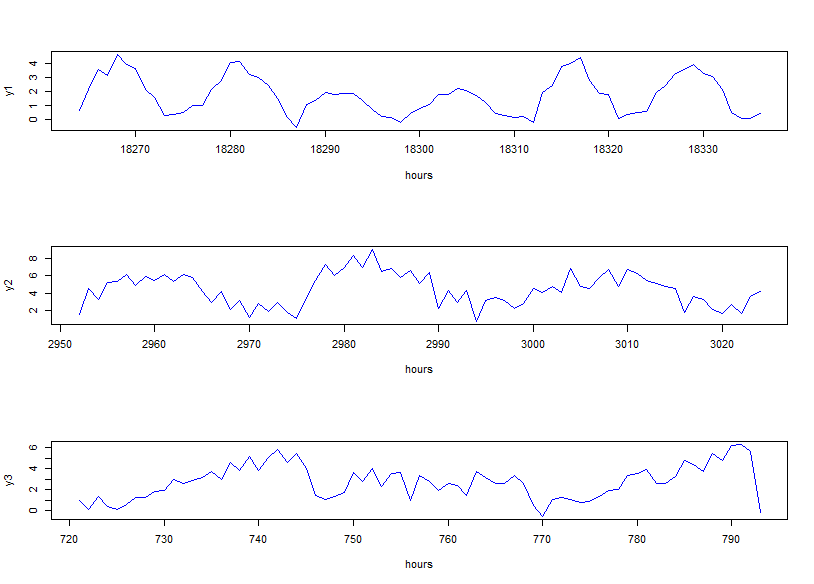
\includegraphics[scale=0.7]{Figures/Anomalies}
	\decoRule
	\caption[Synthetic Anomalies]{Synthetic Anomalies \parencite{own}}
	\label{fig:anomalies}
\end{figure}

For the supervised learning approach the dataset was also labelled. In each case the whole day was marked as an anomaly. In total 30 anomalous days were embedded into the dataset, this corresponds to 1.5 percent of anomalous datapoints.

\subsection{Neural Networks}
In the first experiment, a CNN was tested against a RNN in a supervised and also in an unsupervised fashion. As RNN, the type GRU was chosen. As some first attempts showed, that it showed sufficient results with improved computation time compared to the more complex LSTM. 

For the supervised learning approach, the chosen architecture can be seen in table \ref{Tab:Supervised Learning1}. The architecture with two hidden layers, first presented in Section \ref{Anomaly Detection on Univariate Time Series}, served as example for the RNN. Supplementary, the CNN was built to match the number of layers used for the RNN, where each convolutional layer was followed by a max-pooling layer (explained in Section \ref{CNN}.     

\begin{table}[h]
\caption{Supervised Learning}
	\begin{center}
		\begin{tabular}{ | c | c | c | c |}
			\hline
			\thead{} & \thead{Input} & \thead{NN-Architecture} & \thead{Output} \\
			\hline
			\thead{CNN} &  120 past datapoints  & \makecell{2 1D-Convolutional Layers \\ 2 Max-Pooling Layers \\ 1 Dense Layer}  & \makecell{1 Dense Layer \\ with Sigmoid Activation}   \\
			\hline
			\thead{RNN} &  120 past datapoints  & \makecell{2 GRU Layers \\ 1 Dense Layer}  & \makecell{1 Dense Layer \\ with Sigmoid Activation}  \\
			\hline
		\end{tabular}
		\label{Tab:Supervised Learning1}
	\end{center}
\end{table}

 
The architecture used for the unsupervised learning approach, displayed in table \ref{Tab:Unupervised Learning1}, looked very similar to the architecture of the supervised approach. The main difference between the two architectures was that the CNN was not built as a sequential model, because the used software does not support such an architecture. Instead of having one output layer, the CNN had to be designed with five parallel output layers, each predicting one time series \footnote{More detailed summaries of the models can be found in appendix \ref{AppendixA}}. In comparison, the RNN has just one output layer with 5 neurons, each used to predict a time series.    

\begin{table}[h]
	\caption{Unupervised Learning}
	\begin{center}
		\begin{tabular}{ | c | c | c | c |}
			\hline
			\thead{} & \thead{Input} & \thead{NN-Architecture} & \thead{Output} \\
			\hline
			\thead{CNN} &  120 past datapoints  & \makecell{2 1D-Convolutional Layers \\ 2 Max-Pooling Layers }  & \makecell{ 5 Dense Layers with \\ 1 regression outputs}   \\
			\hline
			\thead{RNN} &  120 past datapoints  & \makecell{2 GRU Layers}  & \makecell{ 1 Dense Layers with \\ 5 regression outputs}  \\
			\hline
		\end{tabular}
	\label{Tab:Unupervised Learning1}
	\end{center}
\end{table}

\subsubsection{Learning}
The learning on the data was done using a so called generator function, which iterates over the dataset in predefined steps. The generator function takes the following parameters:

\begin{itemize}
	\item Lookback - How many data points are considered
	\item Step - How the data is sampled
	\item Delay - How many time steps in the future is the target
	\item Batch Size - The number of samples per batch
\end{itemize}

For this experiment, the parameter lookback was set to 120 data points in the past, which represent the last 5 days. The parameters step and delay were set to one and as batch size 128 was chosen. This setup can be described as follows: There are 128 ordered samples taken from the the whole dataset. Each of these samples consist of 120 data point of past data. With the step parameter set to one, there is not further subsampling done. With delay set to one, the task for the neural network is to predict the next data point in the future per sample for each variable in the data set. This task is done simultaneously for all samples of batch, which speeds up training.

\subsection{Results}

Inference time and F1-Score are, for all models, calculated on the same test dataset. As the initial dataset, it consists of 48000 datapoints, with 30 anomalous days embedded. For the supervised approach using a RNN, no F1-Score is reported, as the model, just like the trivial null classifier, always predicted no anomaly. Since the anomalies span over a whole day, for all approaches, the results were averaged per day. Resulting in normal or anomalous days. The reported F1-Score was finally calculated on this data. 


\begin{table}[h]
	\caption{Results}
	\begin{center}
		\begin{tabular}{ | c | c | c | c |}
			\hline
			\thead{} & \thead{F1-Score} & \thead{Training Time} & \thead{Inference Time} \\
			\hline
			\thead{CNN Supervised} &  0.991388  & 169s  & 422s   \\
			\hline
			\thead{RNN Supervised} &  -  & 967s   & 952s   \\
			\hline
			\thead{CNN Unsupervised} & 0.9989817  & 129s   & 435s   \\
			\hline
			\thead{RNN Unsupervised} &  0.9979613  & 300s   & 793s   \\
			\hline
		\end{tabular}
		\label{Tab:Results1}
	\end{center}
\end{table}

From the table \ref{Tab:Results1}, it can be seen that the supervised learning approach takes longer to train. This can be explained by the fact that a CNN must first learn the patterns and only then begins to recognise the anomalies. \textcolor{red}{Further, it shows that despite promising results when training, the trivial null classifier achieves a higher F1-Score than the supervised CNN approach.}
The best score was achieved with a CNN applied in an unsupervised fashion. The CNN reported just one false negative and a false positive, compared to one false negative and two false positives of the RNN.

\newpage

\section{Experiment 2}
In a second experiment, a real dataset was used as base. The anomalies were embedded manually. Since, the unsupervised approach with RNN in Experiment 1 proved useless it was not included in the second experiment. Since the anomalies in training and test set were looked very similar in Experiment 1, the supervised approach with the CNN was able to recognize some of the anomalies. In the second approach, it should be investigated if this is approach could be of any use, if the anomalies consist of a hitherto unknown pattern.

\subsection{Dataset}
The dataset used was derived from the "Appliances Energy Prediction Dataset" available on the UCI Machine Learning Repository. The dataset consists of 9 room temperatures (T1 to T9) and corresponding humidity levels, energy in use of ligth and appliances, two random variables for testing regression models as well as six variables containing weather information. The dataset consists of 19735 datapoints, where 6 datapoints are drawn per hour. Of the available variables only 10 variables were used for the anomaly detection task. The variables used are 5 room temperatures, energy use, outside temperature, air pressure and wind speed. The variables were selected because they show a dependency. For example, a high outside temperature and energy use result in high temperatures in the different rooms. Figure \ref{fig:temp_dataset} provides an insight on the used dataset.


\begin{figure}[h]
	\centering
	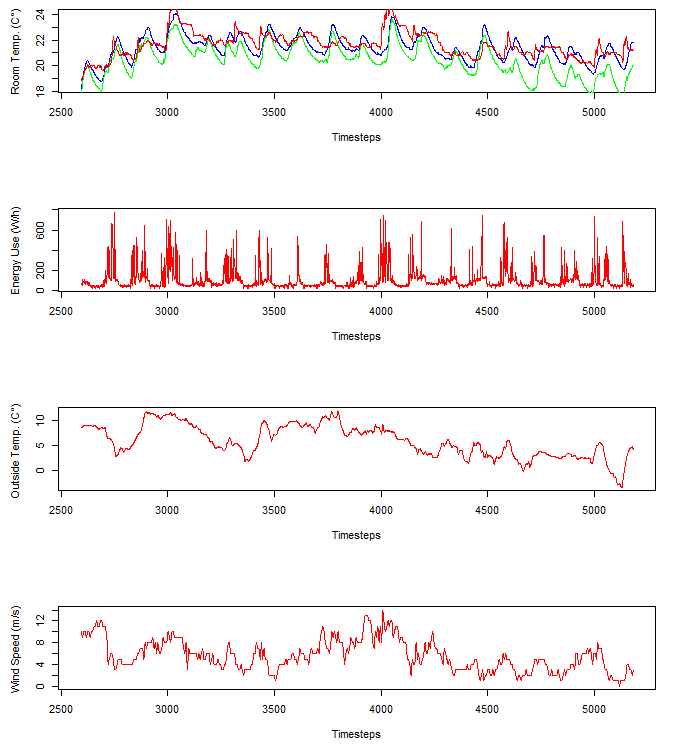
\includegraphics[scale=0.6]{Figures/temp_dataset}
	\decoRule
	\caption[Temperature Dataset]{Appliances Energy Prediction Dataset \parencite{Own or UCI???}}
	\label{fig:temp_dataset}
\end{figure}

\subsubsection{Sampling}
The data set contains datapoints measured between November and May. During this time period, it is observed, that the base temperature steadily rises. This poses the problem, that if the model is trained on data from November to March, with April as validation and May as test period, it is biased on the prevailing colder temperatures. To overcome this problem a special sampling technique was applied. In total six samples of the data set were created. A sample was created by randomly drawing one data point per hour over all datapoints. Four of these sample are then used for training, one for validation and one for testing. Using this sampling technique, the model is no longer biased on certain weather conditions but with the drawback, that the test set is not independent of the test and validation set.   

\subsubsection{Anomalies}
Again, the anomalies were embedded manually into the dataset. The anomalies are of type level shift, deviant cycles, variaton change and distribution-based aggregate anomaly. The anomalies were embedded into the room temperature variables (T1, T2, and T3) and the energy use variable. Figure \ref{fig:temp_anomalies} shows examples of the mentioned anomalies.

\begin{figure}[h]
	\centering
	\includegraphics[scale=0.7]{Figures/temp_anomalies}
	\decoRule
	\caption[Temperature Dataset Anomalies]{Examples of Embedded Anomalies \parencite{Own}}
	\label{fig:temp_anomalies}
\end{figure}

Since the test dataset only consists of around 3000 data points. It was used 3 times so that it does not have an unusual high density of anomalies. In the first instance, anomalies that only affected one variable were embedded. In the second instance, anomalies, that affected all 3 temperature variables, such as a deviant cycle, were embedded. On top, in the energy use variable, variation change anomalies were embedded.  In the third instance, distribution based anomalies, which affected T1 and T2, were embedded.

\subsection{Neural Networks}
Since the RNN did not show sufficient results in Experiment 1 when given a classification task, it was excluded from Experiment 2. The CNN, however, which had probably learned the patterns of the anomalies, was tested again. Since the anomalies in the training and test set are not as similar anymore as in Experiment 1, it is expected that the CNN classifier performs very poorly. 

\begin{table}[h]
	\caption{Unupervised Learning}
	\begin{center}
		\begin{tabular}{ | c | c | c | c |}
			\hline
			\thead{} & \thead{Input} & \thead{NN-Architecture} & \thead{Output} \\
			\hline
			\thead{CNN} &  288 past datapoints  & \makecell{3 1D-Convolutional Layers \\ 1 Max-Pooling Layers }  & \makecell{ 4 Dense Layers with \\ 1 regression outputs}   \\
			\hline
			\thead{RNN} &  288 past datapoints  & \makecell{3 LSTM Layers}  & \makecell{ 1 Dense Layers with \\ 4 regression outputs}  \\
			\hline
		\end{tabular}
		\label{Tab:Unupervised Learning2}
	\end{center}
\end{table}

Because of the complexity of the dataset, in the second experiment it was decided to use LSTM units instead of GRU in the RNN architecture. LSTM units generally provide more accurate results but use more memory and therefore more computation time. The designed neural network architecture consisted of 3 sequential layers of LSTM layers and one dense layer with four neurons. 
%https://analyticsindiamag.com/lstm-vs-gru-in-recurrent-neural-network-a-comparative-study/  

The CNN was designed as follows, three layers of one-dimensional convolutional layers were used. After the first layer, a max-pooling layer was added, to reduce the feature space and improve computation time. Since the CNN is expected to predict a time series, the feature space was not further reduced through max-pooling layers, since it would negatively affect the accuracy.  

\subsubsection{Learning}
The generator function for this experiment was configured as follows:

\begin{itemize}
	\item Lookback - 288 past data points: 12 days in the past
	\item Step - 1: no further subsampling is done
	\item Delay - 1: the next time step in the future is predicted
	\item Batch Size - 128 samples per batch
\end{itemize}

First experiments were done only using data from T1, T2, T3, energy use and outside temperature to predict T1 to T3 and energy use. However as the result were not satisfactory to predict accurate enough results to find the embedded anomalies, further variables were added for training. Finally, the following variables were used to make predictions: T1 to T5, Appliances and Ligths, Outside Temperature, Air Pressure and Windspeed. As the anomlies, however, were only embedded into 4 out of the 10 variables, only the affected 4 were predicted.


\subsection{Results}
Because the dataset was much more challenging, the reported scores are clearly inferior to Experiment 1. In total there were 13 anomalies to be detected in the test sets. The difference in F1-Score between the CNN and the RNN results from one anomaly which was not recognized by the CNN. However, training the RNN takes over 30 times longer than the CNN.

\begin{table}[h]
	\caption{Results}
	\begin{center}
		\begin{tabular}{ | c | c | c | c |}
			\hline
			\thead{} & \thead{F1-Score} & \thead{Training Time} & \thead{Inference Time} \\
			\hline
			\thead{CNN Unsupervised} & 0.666666 & 172s   & 24s*   \\
			\hline
			\thead{RNN Unsupervised} & 0.727272 & 5420s   & 93s*   \\
			\hline
		\end{tabular}
		\label{Tab:Results2}
	\end{center}
\end{table}
* the inference time reported is on just one instance of the test dataset

The above reported results show the overall performance. Since the dataset was more complex than in the first experiment, the results are investigated further to show how the different architecture performed on the various anomalies and how accurate the predictions were on the different variables. First of all, the average error of the predicted variables are investigated further. The below results are reported from the first test set.

\begin{table}[h]
	\caption{Results}
	\begin{center}
		\begin{tabular}{ | c | c | c | c |}
			\hline
			\thead{} & \thead{CNN} & \thead{RNN} \\
			\hline
			\thead{T1} & 0.2712066° C   & 0.1741582° C    \\
			\hline
			\thead{T2} & 0.5236905° C    & 0.9009765° C    \\
			\hline
			\thead{T3} & 0.3210329° C    & 0.7244096° C    \\
			\hline
			\thead{Appliances} & 29.64146 Wh   & 72.91079 Wh   \\
			\hline
		\end{tabular}
		\label{Tab:Average_error}
	\end{center}
\end{table}

From Table \ref{Tab:Average_error}, it can be seen that the CNN outperforms the RNN on all variables except T1. The RNN, however, performs exceptionally well on T1. Comparing these results to the performance of the different architectures on the first test set





\section{Experiment 3}
